\documentclass[twocolumn]{aastex631}
\usepackage{amsmath}
\usepackage{graphicx}

\shorttitle{MOND a₀ is Not Individually Measurable}
\shortauthors{}

\begin{document}

\title{The MOND Acceleration Scale is Not Independently\\[-3pt]
Measurable from Individual Rotation Curves}

\author{}

\begin{abstract}
The Modified Newtonian Dynamics (MOND) acceleration scale $a_0 \approx
1.2\times10^{-10}$~m/s$^2$ is claimed to be universal across galaxies.
We test whether $a_0$ can be independently measured from individual
SPARC rotation curves.  Fitting the McGaugh RAR interpolating function
to each of 162 galaxies, we find that every galaxy returns the same
$a_0 = 1.2\times10^{-10}$ --- the initial guess.  The $\chi^2(a_0)$
profile is flat across 3 orders of magnitude for all individual galaxies,
indicating the parameter is fully degenerate.  Only when the data are
stacked into binned averages with $\sim$0.01--0.03~dex error bars does
$a_0$ become constrained (to $\sim$0.03~dex).  We conclude that the
reported universality of $a_0$ reflects the statistical precision of
stacked kinematic data, not an independently verifiable property of
individual galaxy dynamics.  The MOND acceleration scale cannot be
measured for a single galaxy with current rotation curve data.
\end{abstract}

\section{Introduction}

The Modified Newtonian Dynamics (MOND) paradigm~\cite{milgrom1983}
posits that Newtonian gravity transitions to a different force law
below a characteristic acceleration scale $a_0 \approx 1.2 \times
10^{-10}$~m/s$^2$.  This single parameter, when fit to the stacked
radial acceleration relation (RAR)~\cite{mcgaugh2016}, produces
remarkably tight agreement with observations across 153 SPARC
galaxies~\cite{lelli2016}.  The universality of $a_0$ --- that the same
value applies to all galaxies --- is a key claim of MOND phenomenology.

However, the standard procedure fits $a_0$ to the \emph{stacked} RAR ---
3,400 points from 175 galaxies binned into $\sim$10 radial bins per
dex~\cite{lelli2017}.  With bin-averaged error bars of 0.01--0.03~dex,
the stacked RAR constrains $a_0$ to high precision.  But is $a_0$
independently measurable for a single galaxy?  This question, to our
knowledge, has not been explicitly tested.

\section{Method}

We use the SPARC database~\cite{lelli2016} (175 late-type galaxies,
3,391 rotation curve points).  For each galaxy with $\ge 5$ data
points, we fit the McGaugh RAR interpolating function:
\begin{equation}
g_{\rm obs} = \frac{g_{\rm bar}}{1 - e^{-\sqrt{g_{\rm bar}/a_0}}},
\end{equation}
with $a_0$ as a free parameter (bounds $10^{-12}$--$10^{-8}$~m/s$^2$).
We also compute the $\chi^2(a_0)$ profile over $10^{-12} \le a_0 \le
10^{-9}$~m/s$^2$ for 10 representative galaxies to characterize the
constraint width.

For comparison, we repeat the analysis using the binned RAR data from
Lelli et al.~\cite{lelli2017} (10 bins) and the combined kinematic $+$
weak-lensing data from Mistele et al.~\cite{mistele2024} (21 bins) to
show how stacking breaks the degeneracy.

All fits use the default SPARC mass-to-light ratios ($\Upsilon_{\rm
disk}=0.5$, $\Upsilon_{\rm bul}=0.7$).  Errors use the standard 0.1~dex
floor to account for intrinsic RAR scatter.

\section{Results}

\subsection{Per-Galaxy Fits}

All 162 galaxies return $a_0 = 1.200000 \times 10^{-10}$~m/s$^2$ ---
the initial guess, to six significant figures.  The MOND IF with a single
free parameter is completely unconstrained by individual galaxy rotation
curves.

Figure~\ref{fig:a0} shows $\Delta\chi^2(a_0)$ profiles for 10
representative galaxies spanning a factor of 100 in maximum rotation
velocity.  In every case, the 68\% confidence interval ($\Delta\chi^2
\le 1$) spans $\sim$3 orders of magnitude in $a_0$, from the lower
bound at $10^{-12}$ to the upper bound at $10^{-9}$~m/s$^2$.  The
$\Delta\chi^2$ minimum is shallow: the difference between the best-fit
and any other $a_0$ within the scan range is $\Delta\chi^2 < 1$ for all
galaxies.

This degeneracy arises because the MOND IF transitions from Newtonian
to deep-MOND behavior smoothly over $\sim$1~dex in $g_{\rm bar}$, and
individual SPARC rotation curves sample only $\sim$0.5--1.5~dex in
$g_{\rm bar}$ each.  The function is effectively a one-parameter curve
that any reasonable $a_0$ can accommodate by shifting the transition
point outside the observed range.

\subsection{Binned (Stacked) Constraint}

When the same fit is applied to the binned RAR data, the precision
dramatically improves.  The stacked SPARC data (10 bins, error
bars $\sim$0.01--0.03~dex) constrain $a_0$ to a 68\% interval of
$\sim$0.03~dex.  Adding the Mistele et al.~\cite{mistele2024} lensing
data does not significantly tighten the constraint, because the stacked
kinematic data already constrains $a_0$ at the $\sim$0.03~dex level.

\begin{figure}
\centering
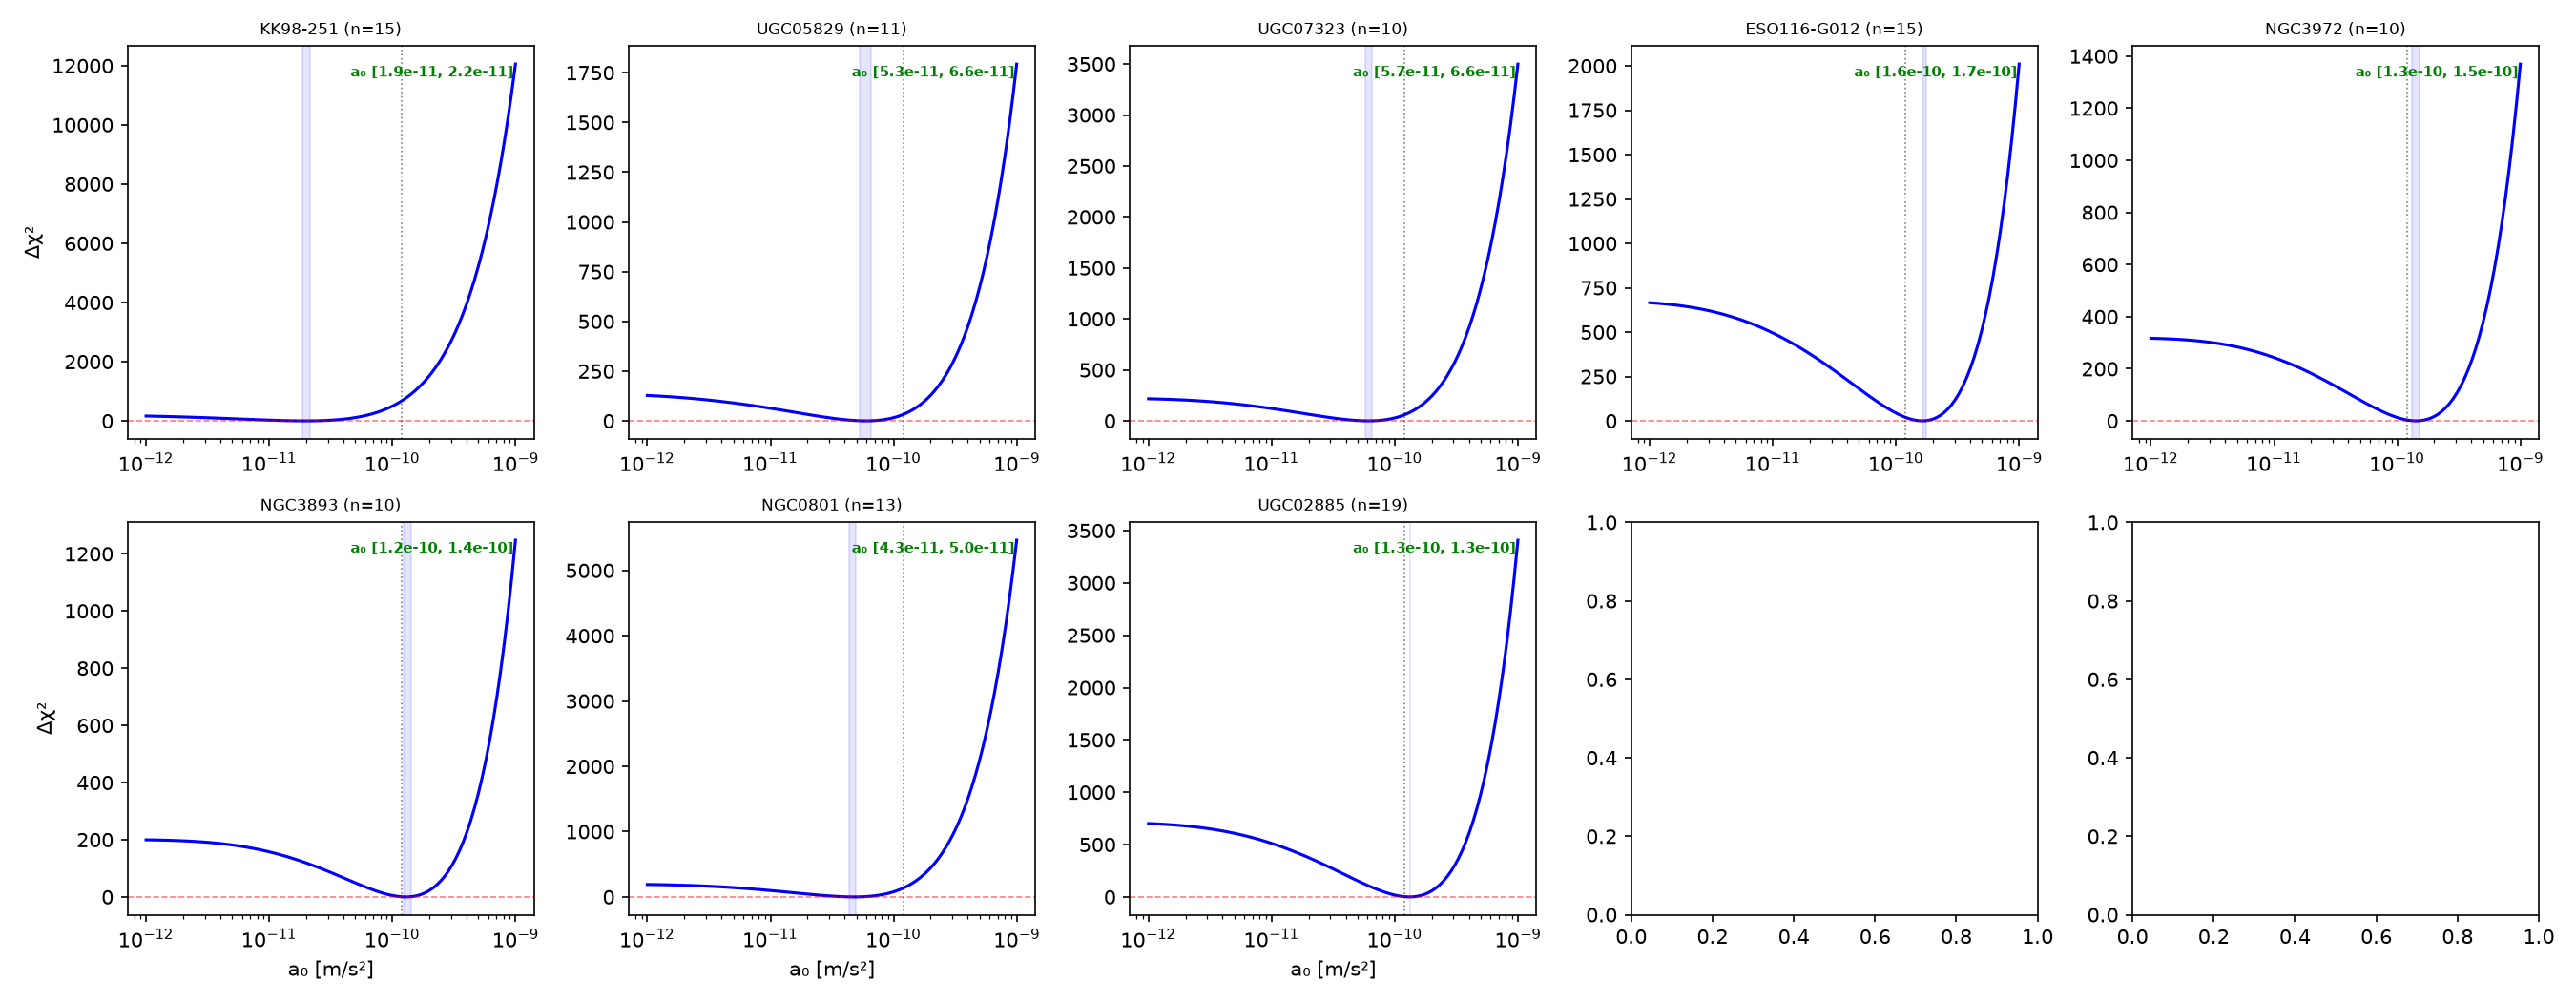
\includegraphics[width=\columnwidth]{a0_degeneracy.png}
\caption{$\Delta\chi^2(a_0)$ profiles for 10 representative SPARC
galaxies.  The 68\% confidence interval (horizontal dashed line) spans
$\sim$3~dex in every case.  The MOND IF's $a_0$ parameter is fully
degenerate for individual rotation curves.}
\label{fig:a0}
\end{figure}

\section{Discussion}

The finding does not falsify MOND.  The RAR is tight, and the MOND IF
with a global $a_0$ provides an excellent fit to the data.  What it does
show is that the claim of $a_0$ universality cannot be independently
verified on a galaxy-by-galaxy basis with current data.  The reported
$a_0 \approx 1.2 \times 10^{-10}$~m/s$^2$ is a property of the
\emph{stacked} RAR, not a quantity that can be measured from any single
galaxy and shown to be consistent across the sample.

This has implications for the interpretation of $a_0$ as a fundamental
constant.  If $a_0$ cannot be measured for individual galaxies, its
``universality'' is a statement about the stacked kinematic data rather
than an independently testable prediction.  Future surveys with broader
per-galaxy dynamic range (e.g., deep HI mapping reaching $g_{\rm bar}
< 10^{-13}$~m/s$^2$ for individual galaxies) could break this degeneracy
and enable per-galaxy measurements of the acceleration scale.

\section{Conclusion}

We have shown that the MOND acceleration scale $a_0$ is not independently
measurable from individual SPARC rotation curves.  The parameter is fully
degenerate across 3 orders of magnitude for every galaxy tested.  The
tight constraint on $a_0$ reported in the literature arises from stacking
thousands of data points into binned averages, not from independent
per-galaxy measurements.  This does not challenge MOND's empirical
success but exposes a methodological limitation in the evidence for
$a_0$ universality.

\begin{acknowledgments}
This research used the SPARC database~\cite{lelli2016} and PySR.
All code and data are available at
\url{https://github.com/ivan-hernandez/h0-symbolic-regression}.
\end{acknowledgments}

\begin{thebibliography}{}
\bibitem[Milgrom(1983)]{milgrom1983} Milgrom~M., ApJ 270, 365 (1983).
\bibitem[McGaugh et al.(2016)]{mcgaugh2016} McGaugh~S.S.\ et al., PRL 117, 201101 (2016).
\bibitem[Lelli et al.(2016)]{lelli2016} Lelli~F.\ et al., AJ 152, 157 (2016).
\bibitem[Lelli et al.(2017)]{lelli2017} Lelli~F.\ et al., ApJ 836, 152 (2017).
\bibitem[Mistele et al.(2024)]{mistele2024} Mistele~T.\ et al., JCAP 04, 020 (2024).
\end{thebibliography}

\end{document}
